\documentclass[a4paper,landscape]{article}
\usepackage[utf8]{inputenc}
\usepackage{graphicx}
\usepackage{float}
\usepackage{geometry}
\geometry{margin=1in}
\usepackage{caption}
\usepackage{hyperref}
\usepackage{xcolor}

\title{Data Visualization Portfolio + image generated!!!! maybe a graph}
\author{Alan Copa}
\date{Data Analytics for Finance I \& II, 2024-2025}

\begin{document}

\maketitle

\tableofcontents
\newpage

\section{Introduction}
This portfolio presents a collection of data visualizations created as part of the course Data Analytics for Finance I \& II requirements for the 2024-2025 academic year.

\section{Visualization Tasks}

\subsection{Task 1: Bad/Manipulative Visualization Critique}
\textbf{Description:} A critique of a poorly designed or manipulative visualization, highlighting its flaws and suggesting improvements.

\textbf{Critique:}
[Write your 100-150 word critique here.]

\subsection{Task 2: Improved Bad Visualization}
\textbf{Description:} An improved version of the bad visualization presented in Task 1.

\begin{figure}[H]
    \centering
    % \includegraphics[width=0.8\textwidth]{improved_viz.png} % Replace with your file name
    \caption{Improved version of the bad visualization.}
    \label{fig:improved}
\end{figure}

\textbf{Disclosure:} This graph was generated using OpenAI tools to assist with data analysis and visualization. All data inputs and final outputs were reviewed and validated for accuracy.

\subsection{Task 3: Good Visualization Critique}
\textbf{Description:} A critique of an exceptionally well-designed visualization, highlighting its strengths.

\textbf{Critique:}
[Write your 100-150 word critique here.]

\subsection{Task 4: Climate Change Visualization for Social Media}
\subsubsection{The Ozone Layer: Evidence of Global Environmental Action}

\begin{figure}[H]
    \centering
    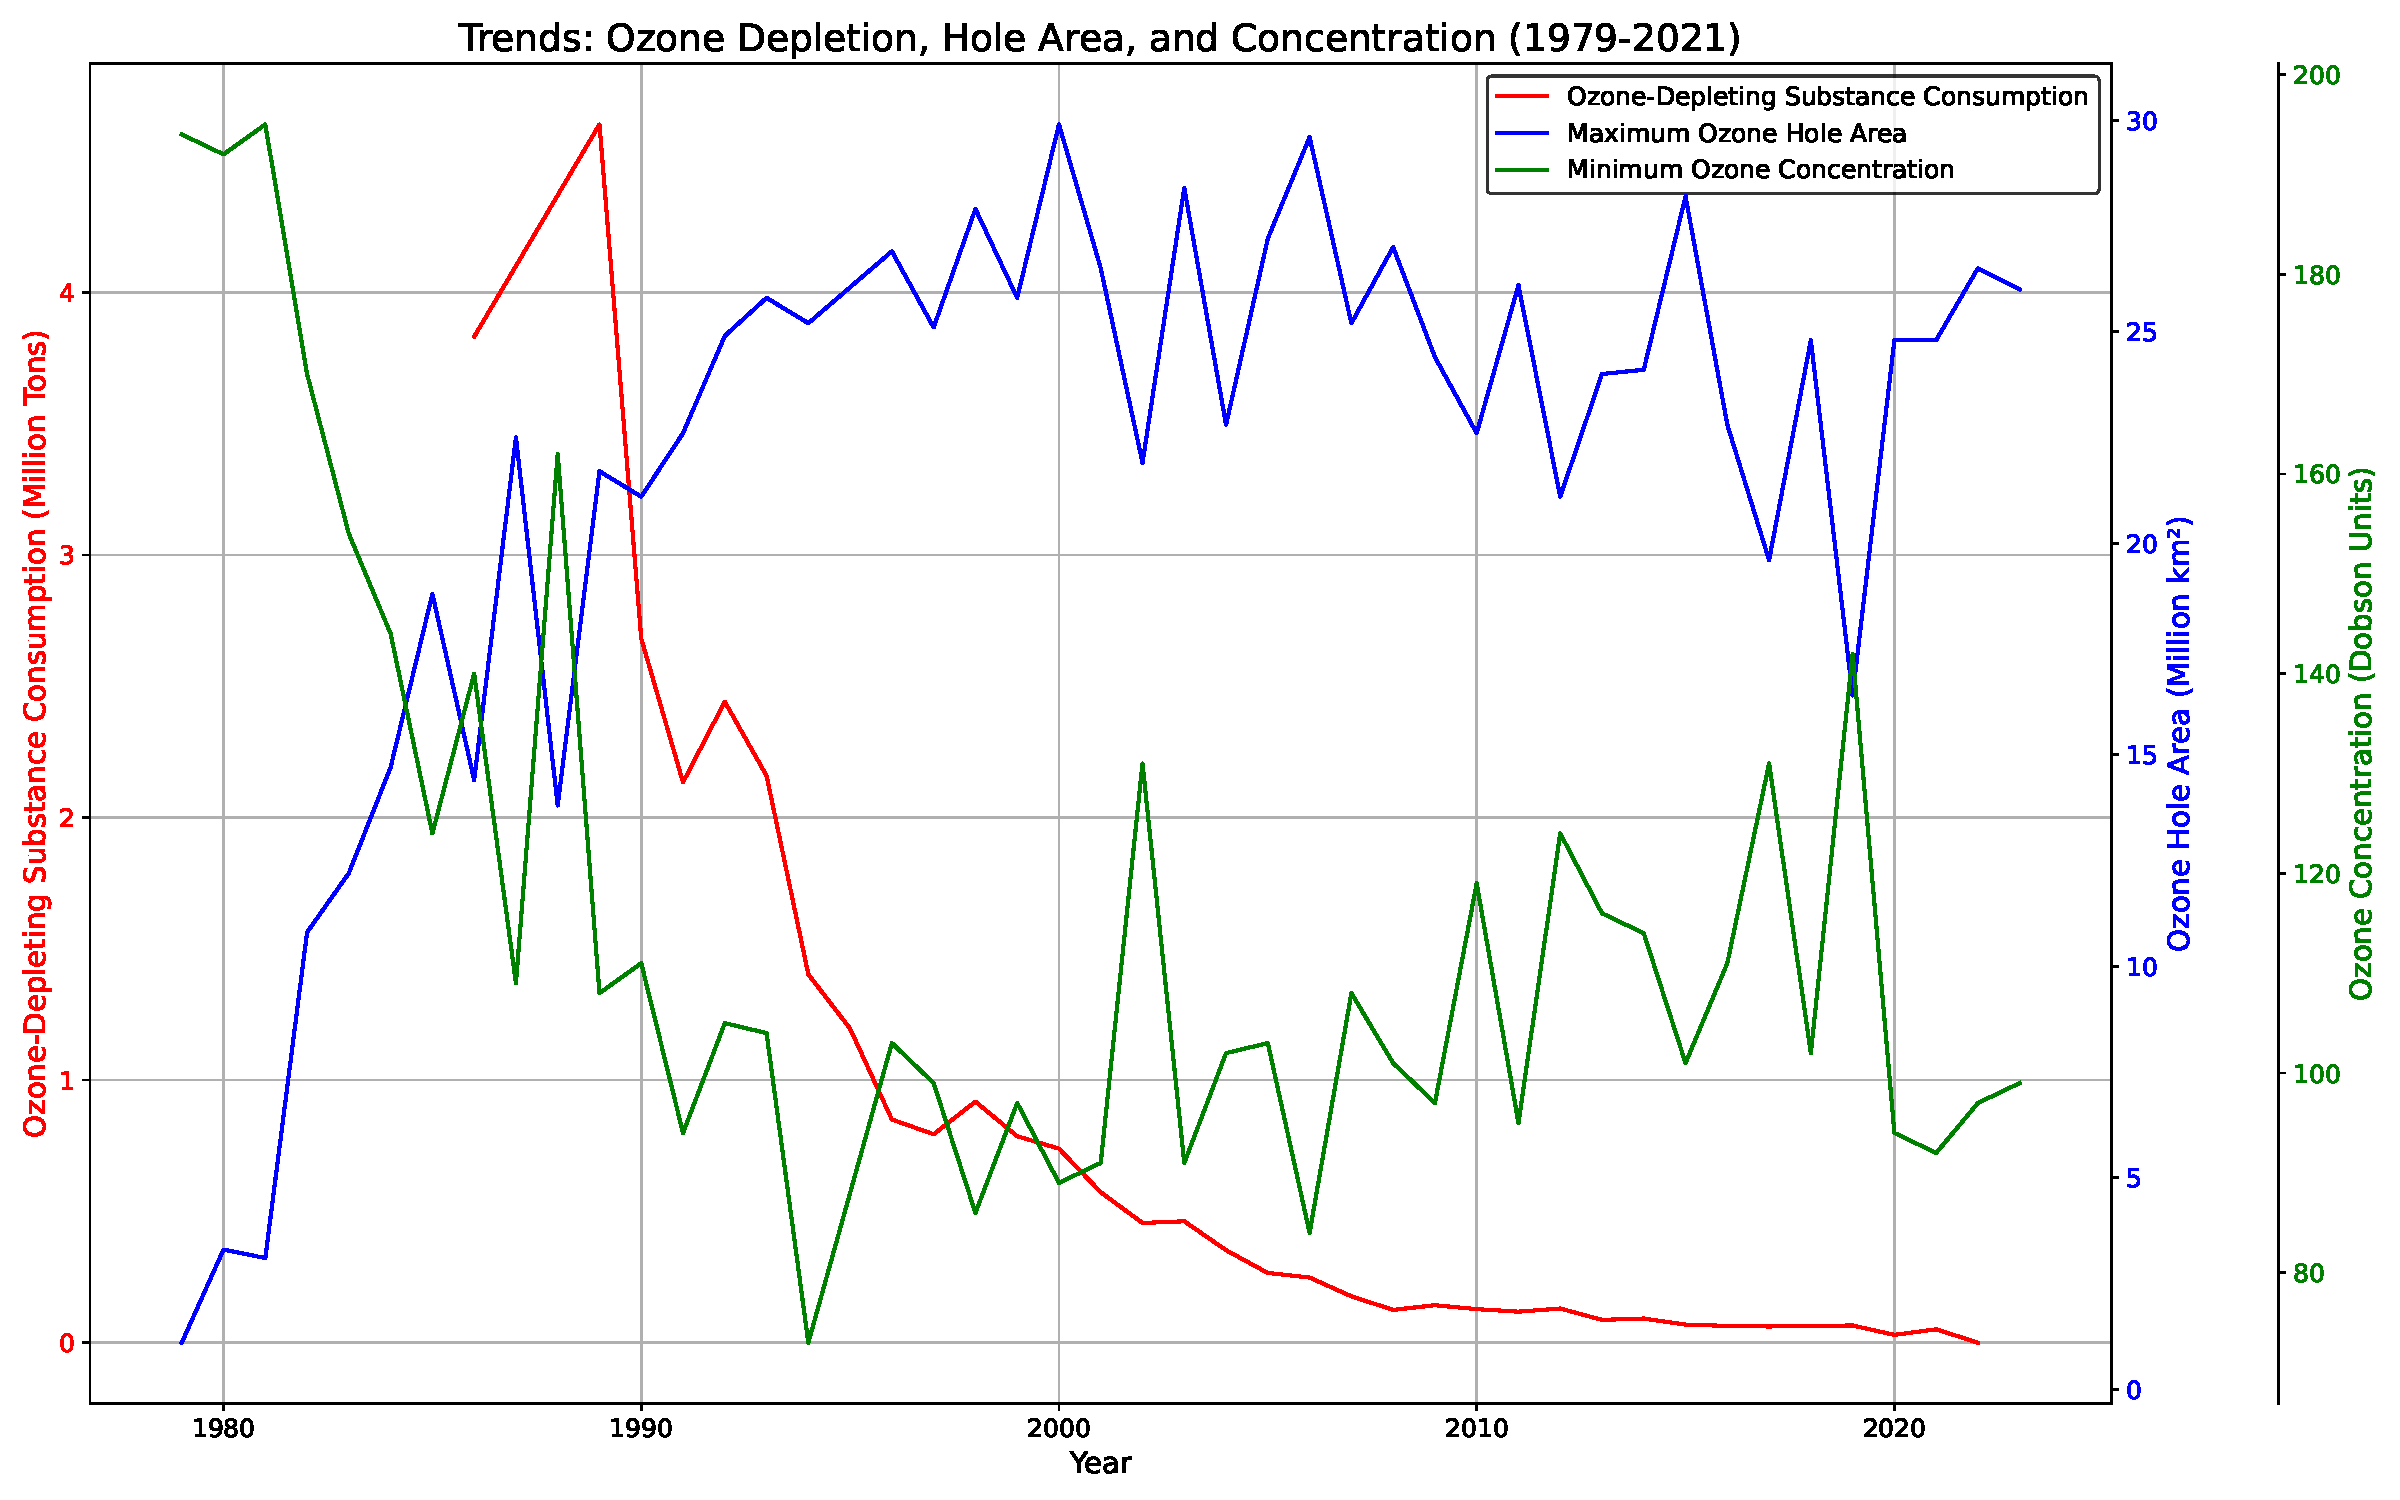
\includegraphics[width=0.8\textwidth]{ozone_data_visualization_t4.pdf} % Replace with your file name
    \caption{Climate change visualization for social media.}
    \label{fig:climate}
\end{figure}

\newpage

\textbf{LinkedIn Post:}
[Write your LinkedIn post here.]

\textbf{Disclosure:} This graph was generated using OpenAI tools to assist with data analysis and visualization. All data inputs and final outputs were reviewed and validated for accuracy.

\subsection{Task 5: Black-and-White Visualization}
\textbf{Description:} A visualization using only black and white, with no shades of gray.

\begin{figure}[H]
    \centering
    % \includegraphics[width=0.8\textwidth]{bw_viz.png} % Replace with your file name
    \caption{Black-and-white visualization.}
    \label{fig:bw}
\end{figure}

\textbf{Disclosure:} This graph was generated using OpenAI tools to assist with data analysis and visualization. All data inputs and final outputs were reviewed and validated for accuracy.

\subsection{Task 6: Visualization with Color as a Key Aesthetic}
\textbf{Description:} A visualization that emphasizes the use of color to convey information.

\begin{figure}[H]
    \centering
    % \includegraphics[width=0.8\textwidth]{color_viz.png} % Replace with your file name
    \caption{Visualization utilizing color as a key aesthetic.}
    \label{fig:color}
\end{figure}

\subsection{Task 14: More Visualizations}
\subsubsection{Measures history of Gravitational Constant G}

\begin{figure}[H]
    \centering
    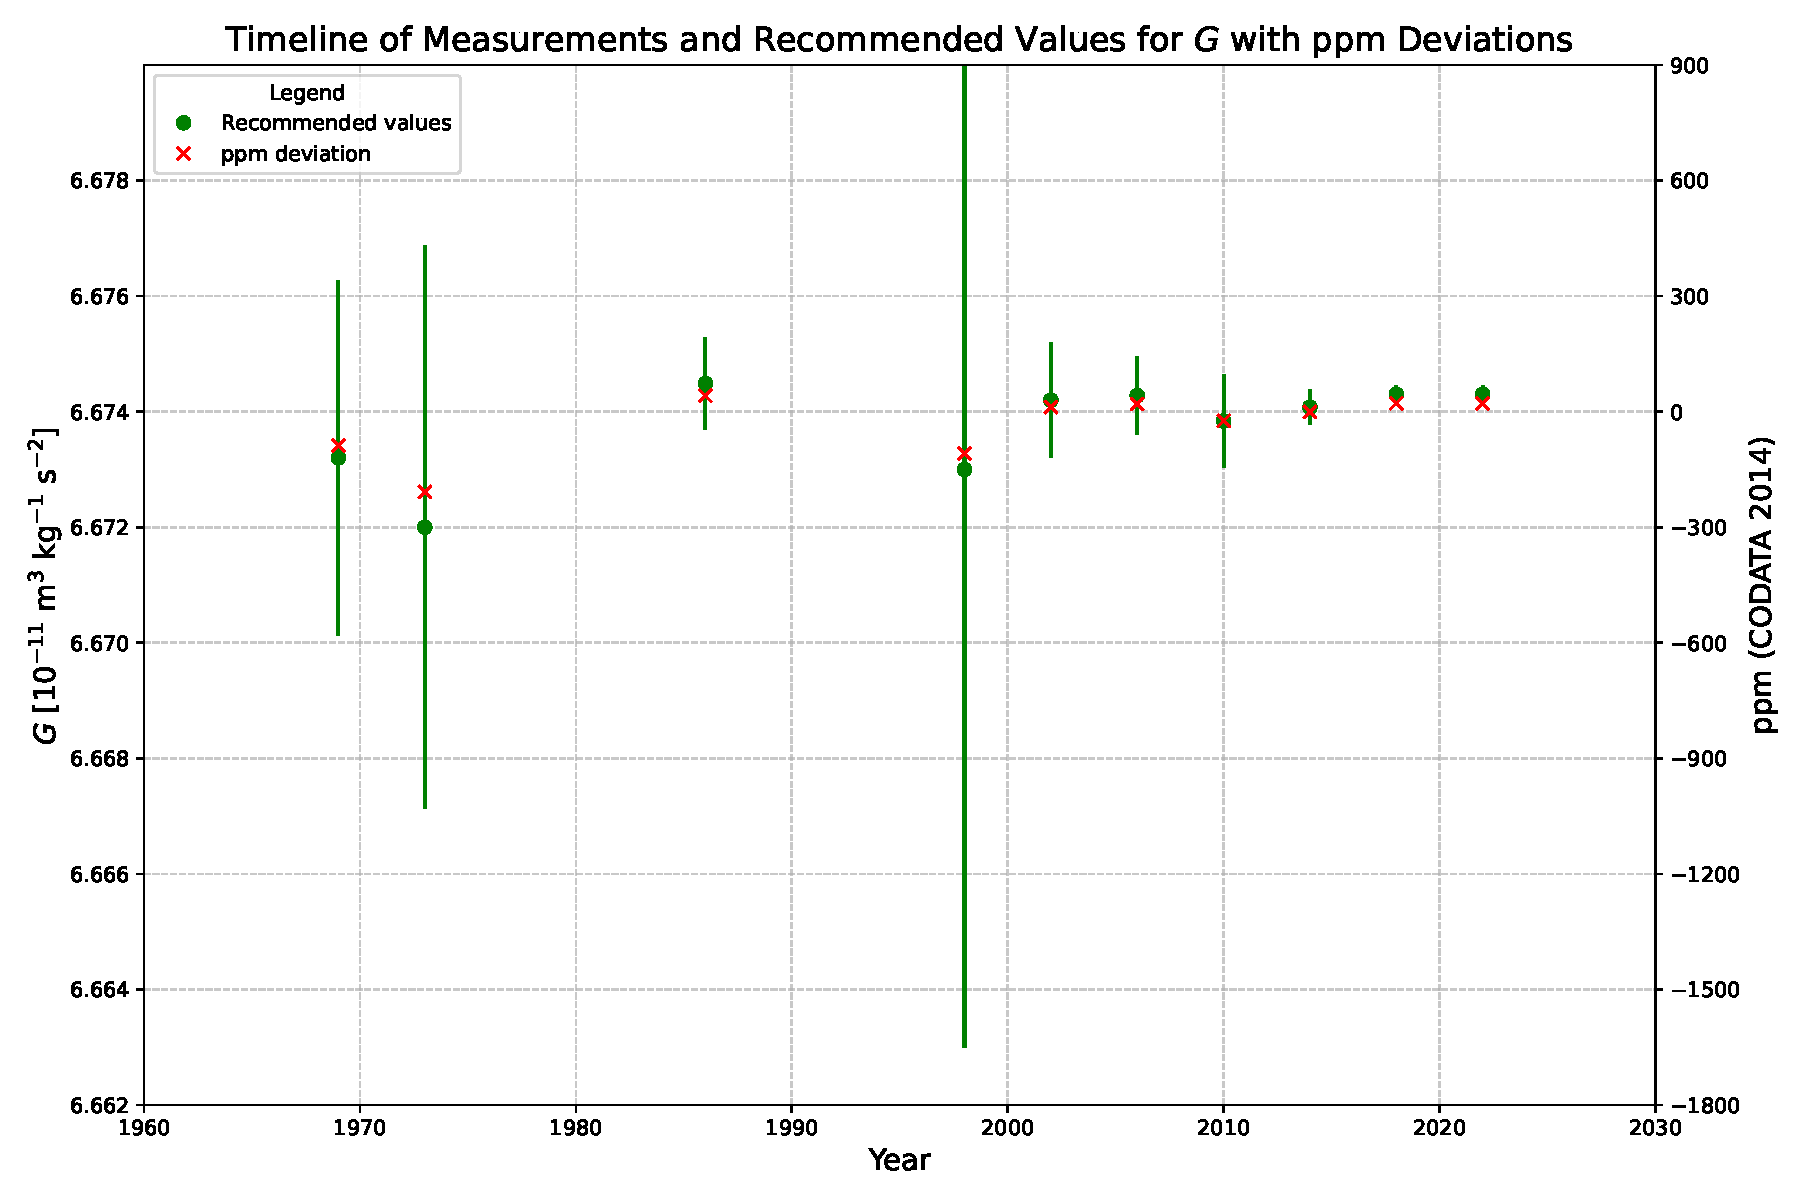
\includegraphics[width=0.8\textwidth]{gravitational_constant.pdf} % Replace with your file name
    \caption{}
    \label{fig:G}
\end{figure}

\subsection{Task 11: Data Map}
\subsubsection{inflation rate}

\begin{figure}[H]
    \centering
    % \includegraphics[width=0.8\textwidth]{?.pdf} % Replace with your file name
    \caption{}
    \label{fig:inflation}
\end{figure}

\textbf{Disclosure:} This graph was generated using OpenAI tools to assist with data analysis and visualization. All data inputs and final outputs were reviewed and validated for accuracy.

\section{References}
\subsection{Data Sources:}
\begin{itemize}
    % \item \href{https://www.kaggle.com/datasets/berkeleyearth/climate-change-earth-surface-temperature-data}{Climate Change: Earth Surface Temperature Data }
    % \item \href{https://www.kaggle.com/datasets/joebeachcapital/global-earth-temperatures/code}{Global Earth Temperatures}
    % \item \href{https://www.kaggle.com/datasets/ulrikthygepedersen/co2-emissions-by-country}{CO2 Emissions by Country}
    \item \href{https://ourworldindata.org/ozone-layer?insight=emissions-of-substances-that-deplete-the-ozone-layer-have-fallen-by-more-than-99#key-insights}{Nasa Sources on Ozone Layer}
    \item \href{https://ourworldindata.org/internet}{Landline Internet subscriptions}
    \item \href{https://en.wikipedia.org/wiki/Gravitational_constant}{Gravitational Constant Data}
\end{itemize}

\subsection{Software and Tools Used:}
% [List all tools, packages, and software used.]
Python Packages
\begin{itemize}
    \item matplotlib, numpy, pandas, os, subprocess, plotly
\end{itemize}
Software
\begin{itemize}
    \item ChatGpt Plus, GPT-4o, My GPTs
\end{itemize}
\textbf{Generative AI Disclosure:}
\begin{itemize}
    \item Task 4: Used ChatGPT Pro to generate Python script for bar chart.
\end{itemize}

\section{Appendix}
\textbf{Screenshots of AI Conversations:}
[Insert screenshots or documentation here.]

\end{document}
